\documentclass{beamer}
\usepackage[utf8]{inputenc}
\usetheme{Madrid}
\usepackage{amssymb}
\usepackage{pifont}
\usepackage{xcolor}
\usepackage{bigints}
\usepackage{mathrsfs}
\definecolor{mblue}{rgb}{0.18,0.21,0.67}
\definecolor{dgreen}{rgb}{0.,0.6,0.}
\newcommand{\cmark}{{\color{dgreen}\ding{52}}}%
\newcommand{\xmark}{{\color{red}\ding{55}}}%
\newcommand{\bmark}{{\color{orange}$\sim$}}%
\newcommand{\arrow}{{{\color{mblue}\ding{220}}}}
\newcommand{\mbold}[1]{\textbf{\color{mblue}#1}}
%\usepackage{marvosym}
\usepackage{soul}

\usepackage{multicol}

\usepackage{amsmath}
\usepackage{cancel}
\DeclareMathOperator*{\argmax}{argmax}
\DeclareMathOperator*{\argmin}{argmin}

% bibliography
\usepackage[backend=bibtex, style=authoryear-comp]{biblatex}
\usepackage{filecontents}
%\newcommand{\customcite}[1]{\citeauthor{#1}, \citetitle{#1}, \citeyear{#1}}
\newcommand{\customcite}[1]{\citeauthor{#1} (\citeyear{#1})}

\bibliography{refs}

\beamertemplatenavigationsymbolsempty
%for backup slides
\newcommand{\backupbegin}{
   \newcounter{finalframe}
   \setcounter{finalframe}{\value{framenumber}}
}
\newcommand{\backupend}{
   \setcounter{framenumber}{\value{finalframe}}
}


\AtBeginSection[
  {\frame<beamer>{\frametitle{Outline}   
    \tableofcontents[currentsection,currentsection]}}%
]%
{
  \frame<beamer>{ 
    \frametitle{Outline}   
    \tableofcontents[currentsection,currentsection]}
}


\title[NumKin 2019]{Exponential methods for solving hyperbolic problems with application to kinetic equations}
%\subtitle{Optimisation de WENO pour Vlasov-Poisson}
\author[J. Massot]{N. Crouseilles \inst{1,2} \and L. Einkemmer \inst{3} \and \underline{J. Massot} \inst{2,1}}
\institute[IRMAR]{\inst{1} Inria Rennes -- Bretagne Atlantique \and \inst{2} IRMAR, Université de Rennes \and \inst{3} University of Innsbruck}
\date{October 17, 2019}

% \defbeamertemplate*{title page}{customized}[1][]
% {
%   \vfill
%   {\usebeamerfont{title}\inserttitle}\par
%   {\usebeamerfont{subtitle}\usebeamercolor[bg]{subtitle}\insertsubtitle}\par
%   \bigskip
%   \vfill
%   \hfill\usebeamerfont{author}\insertauthor\par\par
%   \hfill\textcolor{black}{Encadré par~: Anaïs Crestetto\\\hfill et Nicolas Crouseilles}\par
%   \vfill
%   \hfill\usebeamerfont{date}\insertdate
% }

\begin{document}

\begin{frame}[plain]
  \titlepage
\end{frame}

\begin{frame}{Outline}
  \tableofcontents
\end{frame}

\section{Motivation for Vlasov-Poisson equations}
%%%%%%%%%%%%%%%%%%%%%%%%%%%%%%%%%%%%%%%%%%%%%%%%%%%%%%%%%%%%%%%%%%%%%%%%%%%%%%%

\begin{frame}{Vlasov-Poisson equations 1D$\times$1D}
  Our model: a non-linear transport in $(x,v)\in\Omega\times\mathbb{R}$ of an electron density distribution $f=f(t,x,v)$:
  $$
    \begin{cases}
      \partial_t f + v\partial_x f + E\partial_v f = 0 \\
      \partial_x E = \int_{\mathbb{R}} f\,\mathrm{d}v - 1
    \end{cases}
  $$

  \textbf{\color{mblue} Motivation:}
  \begin{itemize}
    \item We want high order methods in $(x,v)$
    \item We want high order methods in time $t$:
      \begin{itemize}
        \item Splitting methods: could have a lot of steps
        \item Runge-Kutta methods: stability constraints (CFL condition)
          \begin{itemize}
            \item The most restrictive CFL condition is associated with the linear part ($\partial_tf + v\partial_x f=0$)
          \end{itemize}
      \end{itemize}
    \end{itemize}
    \arrow We want to propose a compromise: exponential integrators.
\end{frame}
%-------%
\begin{frame}{Vlasov-Poisson equations 1D$\times$1D}
  Fourier transform in $x$ direction of Vlasov, amenable to exponential integrators:
  $$
    \partial_t\hat{f} + ikv\hat{f} + \widehat{E\partial_v f} = 0
  $$
  
  Vlasov is of the form:
  $$
    \dot{u} = iau + F(u)
  $$
  Variation of constant: $\partial_t(e^{-iat}u) = e^{-iat}F(u)$. No more CFL in $x$ of the form $\Delta t\leq \sigma\frac{\Delta x}{v_\text{max}}$ with $[-v_\text{max},v_\text{max}]\equiv\mathbb{R}$.

  Time integration:
  $$
    u(t_n+\Delta t) = \exp(ia\Delta t)u(t_n) + \int_0^{\Delta t}\exp(ia(\Delta t-s))F(u(t_n+s))\,\mathrm{d}s
  $$
  with $\Delta t>0$, $t_n = n\Delta t$ with $n\in\mathbb{N}$

  Linear part is exact! \cmark
\end{frame}
%-------%
\begin{frame}{Idea of exponential integrators}
  \textbf{\color{mblue} 2 classes of methods:}
  \begin{description}
    \item[\textbf{exponential Runge-Kutta:}] solve exactly what we can, and interpolate the rest. For example first order exponential Euler method:
      $$
        u(t_n+\Delta t) \approx u^{n+1} = e^{-ia\Delta t}u^n + \Delta t\varphi_1(ia\Delta t)F(u^n)
      $$
      where $\varphi_1(z) = \dfrac{e^z - 1}{z}$
      \begin{thebibliography}{9}
        \setbeamertemplate{bibliography item}[article]
        \bibitem{a} \customcite{Hochbruck:2010}
      \end{thebibliography}
    \item[\textbf{Lawson:}] Change of variable: $v(t)=e^{-iat}u(t)$, we solve with a RK method: $\dot{v} = \tilde{F}(t,v) = e^{-iat}F(e^{iat}v(t))$

      For example, Lawson Euler method:
      $$
        v(t_n+\Delta t)\approx v^{n+1} = v^n + \Delta t e^{-iat_n}F(e^{iat_n}v^n)
      $$
      or as an expression of $u$:
      $$
        u^{n+1} = e^{-ia\Delta t}u^n + \Delta te^{ia\Delta t}F(u^n)
      $$
      \begin{thebibliography}{9}
        \setbeamertemplate{bibliography item}[article]
        \bibitem{a} \customcite{Isherwood:2018}
      \end{thebibliography}
  \end{description}
\end{frame}

\section{Linear analysis}
%%%%%%%%%%%%%%%%%%%%%%%%%%%%%%%%%%%%%%%%%%%%%%%%%%%%%%%%%%%%%%%%%%%%%%%%%%%%%%%
\begin{frame}{Reminder of stability tools}
  \only<1>{
    If we want to study stability of:
    $$
      \partial_t u + \partial_x u = 0
    $$
    with centered scheme (CD2) $(\partial_xu)_j \approx \frac{1}{2\Delta x}(u_{j+1}-u_{j-1})$. After a Fourier transform (\emph{von Neumann analysis}):
    $$
      \dot{u} + i\frac{\sin(k\Delta x)}{\Delta x}u = 0
    $$
    Explicit Euler method in time: we have to stretch \mbold{eigenvalues} (or \mbold{Fourier symbol}) of CD2 into explicit Euler \mbold{stability domain}.
  } \only<2>{
    \begin{figure}\centering
      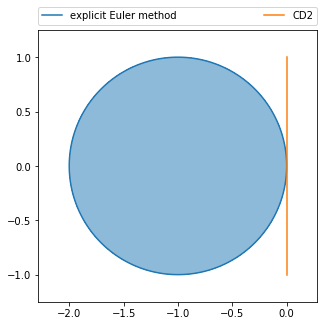
\includegraphics[height=0.8\textheight]{img/cfl_example.png}
    \end{figure}
  }
\end{frame}
%-------%
\begin{frame}{From linear Vlasov equation to toy model}
  Linear Vlasov equation:
  $$
    \partial_t f + a\partial_x f + b\partial_v f = 0
  $$
  Fourier transform in $x$, CD2 in $v$ plus a Fourier transform in $v$, formally:
  $$
    \frac{\mathrm{d}f}{\mathrm{d}t} + iak f + b\frac{i\sin(\varphi)}{\Delta x}f = 0
  $$
  \mbold{Toy model:}
  $$
    \dot{u} + iau + \lambda u = 0
  $$
  with $a\in\mathbb{R}$, $\lambda\in\mathbb{C}$ (diffusive scheme for example).

  $\lambda$ is the Fourier symbol (or eigenvalues) of FD method to approximate $\partial_vf$.
\end{frame}
%-------%
\begin{frame}{Phase discretization}
  In $v$ direction we use a FD method:
  \begin{itemize}
    \item CD2 (centered difference of order 2): $(\partial_v f)(v_j)\approx \dfrac{f_{j+1}-f_{j-1}}{2\Delta v}$
    \item WENO5 (weighted essentially non-oscillatory of order 5):
      \begin{itemize}
        \item WENO5: non linear scheme: \st{Von Neumann analysis}
        \item LW5 (linearized WENO5): linear scheme (this is Lagrange interpolation of order 5)
      \end{itemize}
      $$
        (\partial_vf)(v_j)\approx\frac{1}{\Delta v}\left(-\frac{1}{30}f_{j-3} + \frac{1}{4}f_{j-2} - f_{j-1} + \frac{1}{3}f_j + \frac{1}{2}f_{j+1} - \frac{1}{20}f_{j+2}\right)
      $$

\begin{thebibliography}{9}
  \setbeamertemplate{bibliography item}[article]
  \bibitem{Wang:2007} \customcite{Wang:2007}
  \bibitem{Motamed:2010} \customcite{Motamed:2010}
\end{thebibliography}

  \end{itemize}
\end{frame}
%-------%
\begin{frame}{Fourier symbols}
  \begin{figure}\centering
    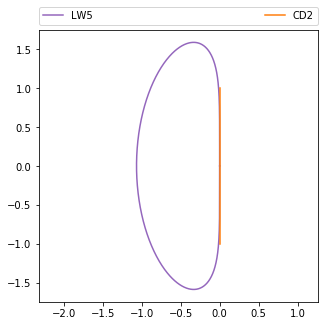
\includegraphics[height=0.8\textheight]{img/weno.png}
  \end{figure}
\end{frame}

\subsection{Lawson methods}
%------------------------------------------------------------------------------
\begin{frame}{Lawson methods stability domain}
  For our toy model:
  $$
    \dot{u} = iau + \lambda(u)
  $$
  Change of variable: $v(t) = e^{-iat}u(t)$
  $$
    \dot{v} = e^{-iat}\lambda e^{iat}v
  $$
  Apply a Runge-Kutta method to compute stability function of Lawson method:
  $$
    v^{n+1} = \underbrace{p(\lambda\Delta t)}_{\text{stability function of RK}}v^n
  $$
  \emph{i.e.}:
  $$
    u^{n+1} = \overbrace{p(\lambda\Delta t)e^{-ia\Delta t}}^{\text{stability function of Lawson}}u^n
  $$
  Stability domain: $\mathcal{D}=\left\{z\in\mathbb{C},|p(z)|\leq 1\right\}$ of Lawson method is \textbf{the same} as the underlying Runge-Kutta method \textbf{because} $ia\in i\mathbb{R}$
\end{frame}
%-------%
\begin{frame}{Considered $Lawson(RK(s,p))$ methods}
  \begin{figure}\centering
    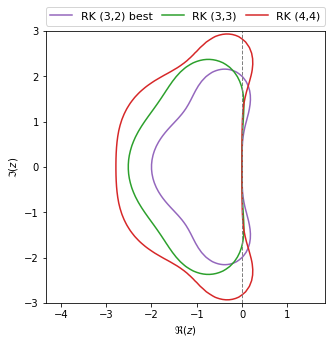
\includegraphics[height=0.8\textheight]{img/rk_sd.png}
  \end{figure}
\end{frame}
%-------%
\begin{frame}{Lawson methods -- CD2}
  For stability between a Lawson method and CD2, we solve:
  $$
    |p(iy)| = 1,\quad y\in\mathbb{R}
  $$
  \begin{table}
    \centering
    \begin{tabular}{|c|c|c|c|}
      \hline
      Methods & Lawson($RK(3,2) \; best$) & Lawson($RK(3,3)$) & Lawson($RK(4,4)$) \\
      \hline
      $y_{\max}$ & $2$ & $\sqrt{3}$ & $2\sqrt{2}$\\
      \hline  
    \end{tabular}
    \caption{CFL number for some Lawson schemes}
  \end{table}
\begin{thebibliography}{9}
  \setbeamertemplate{bibliography item}[article]
  \bibitem{} \customcite{Baldauf:2008}
\end{thebibliography}
\end{frame}
%-------%
\begin{frame}{Lawson methods -- LW5}
  \begin{columns}
    \begin{column}{0.5\textwidth}
      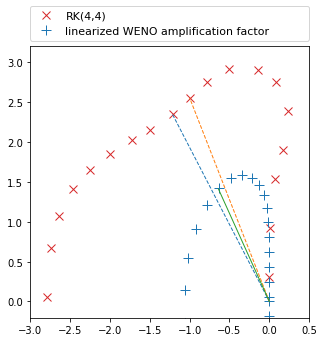
\includegraphics[width=\textwidth]{img/cfl_scheme}
    \end{column}
    \begin{column}{0.5\textwidth}
      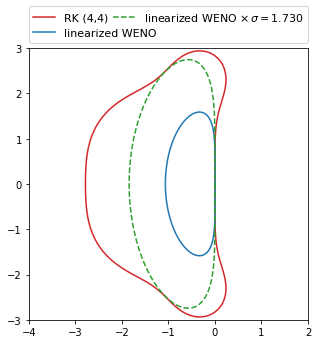
\includegraphics[width=\textwidth]{img/cfl_rk44_weno.png}
    \end{column}
  \end{columns}
\end{frame}
%-------%
\begin{frame}{Lawson methods -- LW5: CFL estimates}
  \begin{table}
    \centering
    \begin{tabular}{|c|c|c|c|}
      \hline
      Methods & Lawson($RK(3,2) \; best$) & Lawson($RK(3,3)$) & Lawson($RK(4,4)$) \\
      \hline
      $\sigma $ & $1.344$ & $1.433$   & $1.73$   \\
      \hline  
    \end{tabular}
    \caption{CFL number for some Lawson schemes.}
  \end{table}
\begin{thebibliography}{9}
  \setbeamertemplate{bibliography item}[article]
  \bibitem{} \customcite{Motamed:2010}
  \bibitem{} \customcite{Lunet:2017}
\end{thebibliography}
\end{frame}

\subsection{Exponential Runge-Kutta methods}
%------------------------------------------------------------------------------

\begin{frame}{Exponential Runge-Kutta methods}
  $$
    \dot{u} = iau + F(u)
  $$
  Example on ExpRK(2,2):
  $$
    \begin{aligned}
      u^{(1)} &= e^{-ia\Delta t}u^n - \Delta t\varphi_1 F(u^n) \\
      u^{n+1} &= e^{-ia\Delta t}u^n - \Delta t\left[ (\varphi_1-\varphi_2)F(u^n) + \varphi_2F(u^{(1)}) \right] 
    \end{aligned}
  $$
  % $$
  %   \begin{aligned}
  %     u^{(1)} &= u^n(1+ia\varphi_{1,2}) + ia\Delta t\varphi_{1,2}F(u^n) \\
  %     u^{n+1} &= u^n(1+ia\Delta t\varphi_1) + \frac{\Delta t}{2}\varphi_1F(u^n)+\frac{\Delta t}{2}\varphi_1F(u^{(1)})
  %   \end{aligned}
  % $$

  Stability function becomes:
  $$
    p_{\text{ExpRK(2,2)}}(z) = \frac{1}{2}\varphi_1\varphi_{1,2}z^2 + (\varphi_1+i\frac{\varphi_1\varphi_{1,2}}{2}a)z + 1 + i\varphi_1a
  $$

  Stability domain depends of $a\Delta t$\dots \xmark
\end{frame}
%-------%
\begin{frame}{}
  \only<1>{
    \begin{figure}\centering
      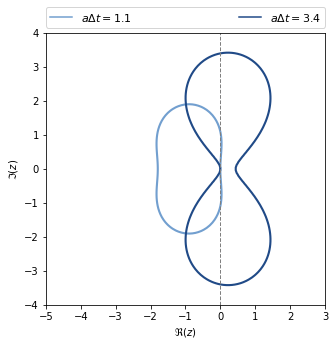
\includegraphics[height=0.7\textheight]{img/expRK22_sd.png}
      \caption{Stability domain of ExpRK(2,2) for $a\Delta t\in\{1.1, 3.4\}$}
    \end{figure}
  }
  \only<2>{
    \begin{figure}\centering
      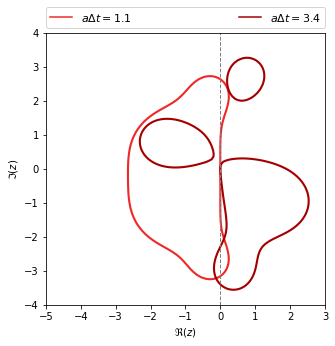
\includegraphics[height=0.7\textheight]{img/CM_sd.png}
      \caption{Stability domain of Cox-Matthews for $a\Delta t\in\{1.1, 3.4\}$}
    \end{figure}
  }
  \only<3>{
    \begin{figure}\centering
      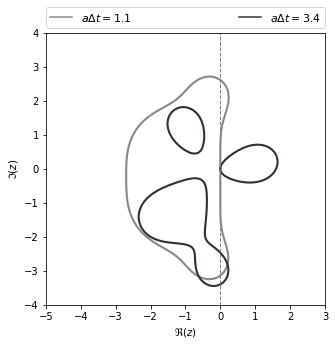
\includegraphics[height=0.7\textheight]{img/K_sd.png}
      \caption{Stability domain of Krogstad for $a\Delta t\in\{1.1, 3.4\}$}
    \end{figure}
  }
  \only<4>{
    \begin{figure}\centering
      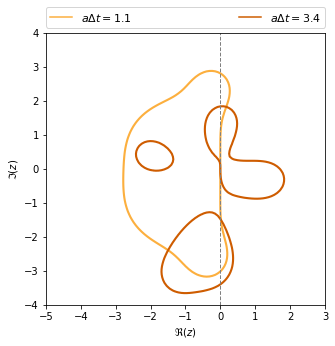
\includegraphics[height=0.7\textheight]{img/HO_sd.png}
      \caption{Stability domain of Hochbruck--Ostermann for $a\Delta t\in\{1.1, 3.4\}$}
    \end{figure}
  }
\end{frame}
%-------%
\begin{frame}{Stability domain informations}
  Fourier symbol must fit in the stability domain of ExpRK method \textbf{for all} values of $a\Delta t\in\mathbb{R}$.
  \begin{description}
    \item[\xmark] Impossible with WENO5 (LW5 Fourier symbol) \begin{description}\item[$\rightarrow$] Numerical test: unstable in very short time\end{description}
    \item[\cmark] Singleton $\{0\}$ is alway in stability domain of ExpRK method for each values of $a\Delta t$
      \begin{description}
        \item[$\rightarrow$] We can try to stabilize CD2
        \item[\xmark] SPOILER: CFL is equal to zero
      \end{description}
  \end{description}
\end{frame}
%-------%
\begin{frame}{ExpRK -- CD2}
  \only<1>{
    \begin{figure}\centering
      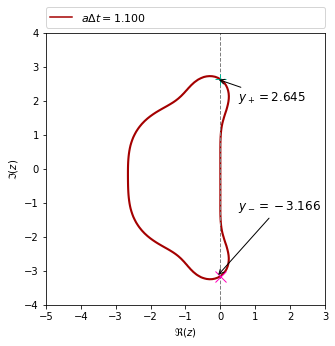
\includegraphics[width=0.5\textwidth]{img/ymax_CM_example1.png}
    \end{figure}
  }
  \only<2>{
    \begin{figure}\centering
      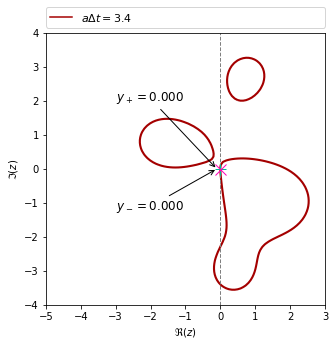
\includegraphics[width=0.5\textwidth]{img/ymax_CM_example2.png}
    \end{figure}
  }
  $y^{exp}_\text{max} = \min(y_+,|y_-|)$ the largest value to stretch $i[-1,1]$ into the stability domain at $a\Delta t$
\end{frame}
%-------%
\begin{frame}{ExpRK -- CD2: CFL number}
  \begin{figure}\centering
    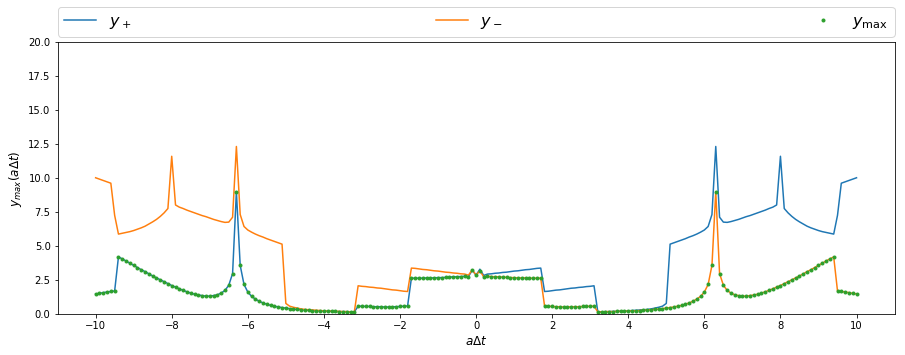
\includegraphics[width=\textwidth]{img/ymax_CM.png}
  \end{figure}
  CFL $y_\text{max} = \min_{a\Delta t}y^{exp}_\text{max}$ is still 0\dots
\end{frame}
%-------%
\begin{frame}{ExpRK -- CD2: Relaxed CFL condition}
  \only<1>{
    $$\mathcal{D}_\varepsilon = \left\{z\in\mathbb{C},|p(z)|\leq1+\varepsilon\right\}$$
    \begin{columns}
      \begin{column}{0.5\textwidth}\centering
        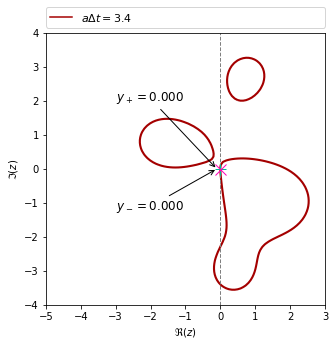
\includegraphics[height=0.6\textheight]{img/CM_sd_ymax_e0p00.png}
        Cox-Matthews stability domain, relaxation $\varepsilon = 0$
      \end{column}
      \begin{column}{0.5\textwidth}\centering
        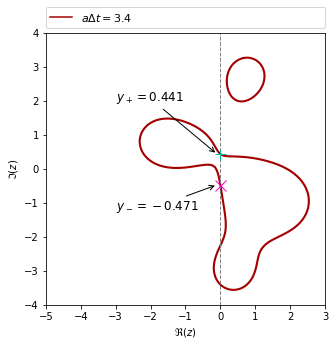
\includegraphics[height=0.6\textheight]{img/CM_sd_ymax_e0p01.png}
        Cox-Matthews stability domain, relaxation $\varepsilon = 10^{-2}$
      \end{column}
    \end{columns}
  }\only<2>{
    \begin{figure}\centering
      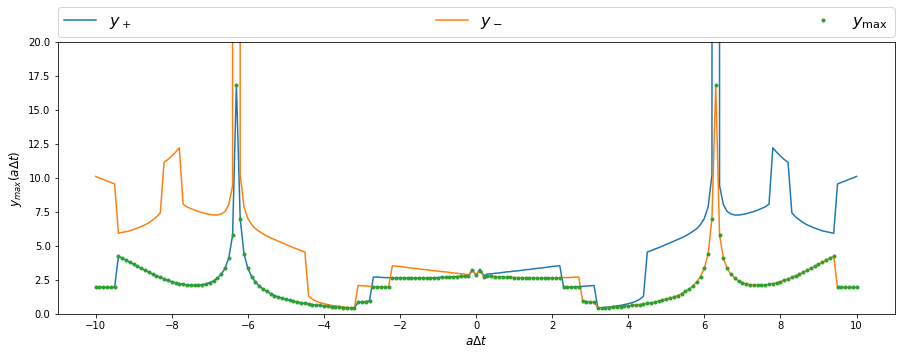
\includegraphics[width=\textwidth]{img/ymax_CM_relax.png}
    \end{figure}
    Relaxed CFL $y_\text{max}(\varepsilon=10^{-2}) \approx 0.450 \neq 0$ ! (but unstable in theory)
  }
\end{frame}
%-------%
\begin{frame}{ExpRK -- CD2: Relaxed CFL estimates}
  \begin{table}
    \centering
    \begin{tabular}{|c|c|c|c|c|}
      \hline
      Methods                                & ExpRK22 & Krogstad & Cox--Matthews & Hochbruck \\
                                             &         &          &               & --Ostermann \\
      \hline
      $y_{\max} (\varepsilon=10^{-3})$ & $0.300$ & $0.100$  & $0.150$      & $0.250$ \\
      \hline
      $y_{\max} (\varepsilon=10^{-2})$ & $0.551$ & $0.200$  & $0.450$      & $0.501$ \\
      \hline  
      $y_{\max} (\varepsilon=10^{-1})$ & $1.001$ & $0.601$  & $1.351$      & $1.702$ \\
      \hline  
    \end{tabular}
    \caption{CFL number, assuming the relaxed stability constraint, for some exponential integrators.}
    It's unstable in theory, in practice, number of iterations is finished, so amplification is controlled.
  \end{table}
\end{frame}

\section{Numerical simulation: Vlasov-Poisson equations}
%%%%%%%%%%%%%%%%%%%%%%%%%%%%%%%%%%%%%%%%%%%%%%%%%%%%%%%%%%%%%%%%%%%%%%%%%%%%%%%

\begin{frame}{Vlasov-Poisson equations}
  $$
    \begin{cases}
      \partial_tf + v\partial_xf + E\partial_vf = 0 \\
      \partial_xE = \int_{\mathbb{R}} f\,\mathrm{d}v - 1
    \end{cases}
  $$

  \mbold{Numerical tools:}
  \begin{itemize}
    \item FFT in $x$ direction
    \item CD2 or WENO5 in $v$ direction
    \item $Lawson(RK(s,p))$ or ExpRK method in time $t$
  \end{itemize}

  \mbold{CFL:} $\Delta t_n \leq \dfrac{C\Delta v}{||E^n||_{\infty}} \leq \dfrac{C\Delta v}{\max_n||E^n||_{\infty}}$ where $C = y_\text{max}$ or $\sigma$ from the linear theory.

  \ 

  We can choose: $\Delta t = \min\left( 0.1 , \dfrac{C\Delta v}{\max_n||E^n||_{\infty}} \right)$
\end{frame}
%-------%
\begin{frame}{Landau damping}
  $$
    f(t=0,x,v) = f_0(x,v) = \frac{1}{\sqrt{2\pi}}e^{-\frac{v^2}{2}}(1+0.001\cos(0.5x))
  $$
  $x\in[0,4\pi]$, $v\in[-8,8]$, $N_x = 81$, $N_v=128$

  \ 

  Because of damping:
  $$
    \max_n||E^n||_{\infty} = ||E^0||_\infty
  $$
  So, we choose $\Delta t = 0.1$ (with $\Delta t = 100$ it is still stable!)
\end{frame}
%-------%
\begin{frame}{Landau damping: numerical results}
  \only<1>{
    \begin{figure}
      \centering
      \resizebox{!}{.7\paperheight}{% GNUPLOT: LaTeX picture with Postscript
\begingroup
  \makeatletter
  \providecommand\color[2][]{%
    \GenericError{(gnuplot) \space\space\space\@spaces}{%
      Package color not loaded in conjunction with
      terminal option `colourtext'%
    }{See the gnuplot documentation for explanation.%
    }{Either use 'blacktext' in gnuplot or load the package
      color.sty in LaTeX.}%
    \renewcommand\color[2][]{}%
  }%
  \providecommand\includegraphics[2][]{%
    \GenericError{(gnuplot) \space\space\space\@spaces}{%
      Package graphicx or graphics not loaded%
    }{See the gnuplot documentation for explanation.%
    }{The gnuplot epslatex terminal needs graphicx.sty or graphics.sty.}%
    \renewcommand\includegraphics[2][]{}%
  }%
  \providecommand\rotatebox[2]{#2}%
  \@ifundefined{ifGPcolor}{%
    \newif\ifGPcolor
    \GPcolorfalse
  }{}%
  \@ifundefined{ifGPblacktext}{%
    \newif\ifGPblacktext
    \GPblacktexttrue
  }{}%
  % define a \g@addto@macro without @ in the name:
  \let\gplgaddtomacro\g@addto@macro
  % define empty templates for all commands taking text:
  \gdef\gplbacktext{}%
  \gdef\gplfronttext{}%
  \makeatother
  \ifGPblacktext
    % no textcolor at all
    \def\colorrgb#1{}%
    \def\colorgray#1{}%
  \else
    % gray or color?
    \ifGPcolor
      \def\colorrgb#1{\color[rgb]{#1}}%
      \def\colorgray#1{\color[gray]{#1}}%
      \expandafter\def\csname LTw\endcsname{\color{white}}%
      \expandafter\def\csname LTb\endcsname{\color{black}}%
      \expandafter\def\csname LTa\endcsname{\color{black}}%
      \expandafter\def\csname LT0\endcsname{\color[rgb]{1,0,0}}%
      \expandafter\def\csname LT1\endcsname{\color[rgb]{0,1,0}}%
      \expandafter\def\csname LT2\endcsname{\color[rgb]{0,0,1}}%
      \expandafter\def\csname LT3\endcsname{\color[rgb]{1,0,1}}%
      \expandafter\def\csname LT4\endcsname{\color[rgb]{0,1,1}}%
      \expandafter\def\csname LT5\endcsname{\color[rgb]{1,1,0}}%
      \expandafter\def\csname LT6\endcsname{\color[rgb]{0,0,0}}%
      \expandafter\def\csname LT7\endcsname{\color[rgb]{1,0.3,0}}%
      \expandafter\def\csname LT8\endcsname{\color[rgb]{0.5,0.5,0.5}}%
    \else
      % gray
      \def\colorrgb#1{\color{black}}%
      \def\colorgray#1{\color[gray]{#1}}%
      \expandafter\def\csname LTw\endcsname{\color{white}}%
      \expandafter\def\csname LTb\endcsname{\color{black}}%
      \expandafter\def\csname LTa\endcsname{\color{black}}%
      \expandafter\def\csname LT0\endcsname{\color{black}}%
      \expandafter\def\csname LT1\endcsname{\color{black}}%
      \expandafter\def\csname LT2\endcsname{\color{black}}%
      \expandafter\def\csname LT3\endcsname{\color{black}}%
      \expandafter\def\csname LT4\endcsname{\color{black}}%
      \expandafter\def\csname LT5\endcsname{\color{black}}%
      \expandafter\def\csname LT6\endcsname{\color{black}}%
      \expandafter\def\csname LT7\endcsname{\color{black}}%
      \expandafter\def\csname LT8\endcsname{\color{black}}%
    \fi
  \fi
    \setlength{\unitlength}{0.0500bp}%
    \ifx\gptboxheight\undefined%
      \newlength{\gptboxheight}%
      \newlength{\gptboxwidth}%
      \newsavebox{\gptboxtext}%
    \fi%
    \setlength{\fboxrule}{0.5pt}%
    \setlength{\fboxsep}{1pt}%
\begin{picture}(7200.00,5040.00)%
    \gplgaddtomacro\gplbacktext{%
      \csname LTb\endcsname%%
      \put(990,440){\makebox(0,0)[r]{\strut{}$0.01$}}%
      \put(990,987){\makebox(0,0)[r]{\strut{}$0.1$}}%
      \put(990,1535){\makebox(0,0)[r]{\strut{}$1$}}%
      \put(990,2082){\makebox(0,0)[r]{\strut{}$10$}}%
      \put(990,2629){\makebox(0,0)[r]{\strut{}$100$}}%
      \put(990,3177){\makebox(0,0)[r]{\strut{}$1000$}}%
      \put(990,3724){\makebox(0,0)[r]{\strut{}$10000$}}%
      \put(990,4272){\makebox(0,0)[r]{\strut{}$100000$}}%
      \put(990,4819){\makebox(0,0)[r]{\strut{}$1\times10^{6}$}}%
      \put(1122,220){\makebox(0,0){\strut{}$0$}}%
      \put(1832,220){\makebox(0,0){\strut{}$5$}}%
      \put(2542,220){\makebox(0,0){\strut{}$10$}}%
      \put(3252,220){\makebox(0,0){\strut{}$15$}}%
      \put(3963,220){\makebox(0,0){\strut{}$20$}}%
      \put(4673,220){\makebox(0,0){\strut{}$25$}}%
      \put(5383,220){\makebox(0,0){\strut{}$30$}}%
      \put(6093,220){\makebox(0,0){\strut{}$35$}}%
      \put(6803,220){\makebox(0,0){\strut{}$40$}}%
    }%
    \gplgaddtomacro\gplfronttext{%
      \csname LTb\endcsname%%
      \put(4950,4646){\makebox(0,0)[r]{\strut{}$\frac{\sigma\Delta v}{||E^n||_{L^\infty}}$}}%
      \csname LTb\endcsname%%
      \put(4950,4426){\makebox(0,0)[r]{\strut{}Effective time step}}%
    }%
    \gplbacktext
    \put(0,0){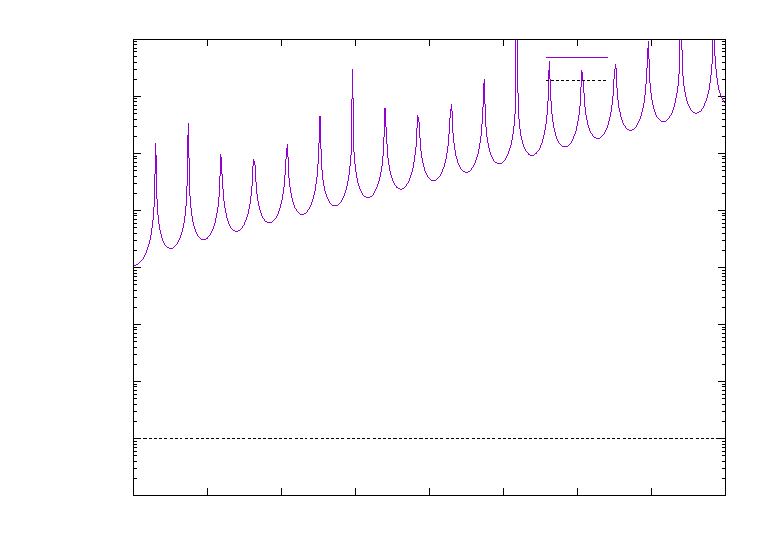
\includegraphics{img/hn}}%
    \gplfronttext
  \end{picture}%
\endgroup
}
      \caption{Landau damping test: time history of the CFL condition (semi-log scale).}
      \label{ld}
    \end{figure}
  }\only<2>{
    \begin{figure}
      \centering
      \resizebox{!}{.7\paperheight}{% GNUPLOT: LaTeX picture with Postscript
\begingroup
  \makeatletter
  \providecommand\color[2][]{%
    \GenericError{(gnuplot) \space\space\space\@spaces}{%
      Package color not loaded in conjunction with
      terminal option `colourtext'%
    }{See the gnuplot documentation for explanation.%
    }{Either use 'blacktext' in gnuplot or load the package
      color.sty in LaTeX.}%
    \renewcommand\color[2][]{}%
  }%
  \providecommand\includegraphics[2][]{%
    \GenericError{(gnuplot) \space\space\space\@spaces}{%
      Package graphicx or graphics not loaded%
    }{See the gnuplot documentation for explanation.%
    }{The gnuplot epslatex terminal needs graphicx.sty or graphics.sty.}%
    \renewcommand\includegraphics[2][]{}%
  }%
  \providecommand\rotatebox[2]{#2}%
  \@ifundefined{ifGPcolor}{%
    \newif\ifGPcolor
    \GPcolorfalse
  }{}%
  \@ifundefined{ifGPblacktext}{%
    \newif\ifGPblacktext
    \GPblacktexttrue
  }{}%
  % define a \g@addto@macro without @ in the name:
  \let\gplgaddtomacro\g@addto@macro
  % define empty templates for all commands taking text:
  \gdef\gplbacktext{}%
  \gdef\gplfronttext{}%
  \makeatother
  \ifGPblacktext
    % no textcolor at all
    \def\colorrgb#1{}%
    \def\colorgray#1{}%
  \else
    % gray or color?
    \ifGPcolor
      \def\colorrgb#1{\color[rgb]{#1}}%
      \def\colorgray#1{\color[gray]{#1}}%
      \expandafter\def\csname LTw\endcsname{\color{white}}%
      \expandafter\def\csname LTb\endcsname{\color{black}}%
      \expandafter\def\csname LTa\endcsname{\color{black}}%
      \expandafter\def\csname LT0\endcsname{\color[rgb]{1,0,0}}%
      \expandafter\def\csname LT1\endcsname{\color[rgb]{0,1,0}}%
      \expandafter\def\csname LT2\endcsname{\color[rgb]{0,0,1}}%
      \expandafter\def\csname LT3\endcsname{\color[rgb]{1,0,1}}%
      \expandafter\def\csname LT4\endcsname{\color[rgb]{0,1,1}}%
      \expandafter\def\csname LT5\endcsname{\color[rgb]{1,1,0}}%
      \expandafter\def\csname LT6\endcsname{\color[rgb]{0,0,0}}%
      \expandafter\def\csname LT7\endcsname{\color[rgb]{1,0.3,0}}%
      \expandafter\def\csname LT8\endcsname{\color[rgb]{0.5,0.5,0.5}}%
    \else
      % gray
      \def\colorrgb#1{\color{black}}%
      \def\colorgray#1{\color[gray]{#1}}%
      \expandafter\def\csname LTw\endcsname{\color{white}}%
      \expandafter\def\csname LTb\endcsname{\color{black}}%
      \expandafter\def\csname LTa\endcsname{\color{black}}%
      \expandafter\def\csname LT0\endcsname{\color{black}}%
      \expandafter\def\csname LT1\endcsname{\color{black}}%
      \expandafter\def\csname LT2\endcsname{\color{black}}%
      \expandafter\def\csname LT3\endcsname{\color{black}}%
      \expandafter\def\csname LT4\endcsname{\color{black}}%
      \expandafter\def\csname LT5\endcsname{\color{black}}%
      \expandafter\def\csname LT6\endcsname{\color{black}}%
      \expandafter\def\csname LT7\endcsname{\color{black}}%
      \expandafter\def\csname LT8\endcsname{\color{black}}%
    \fi
  \fi
    \setlength{\unitlength}{0.0500bp}%
    \ifx\gptboxheight\undefined%
      \newlength{\gptboxheight}%
      \newlength{\gptboxwidth}%
      \newsavebox{\gptboxtext}%
    \fi%
    \setlength{\fboxrule}{0.5pt}%
    \setlength{\fboxsep}{1pt}%
\begin{picture}(7200.00,5040.00)%
    \gplgaddtomacro\gplbacktext{%
      \csname LTb\endcsname%%
      \put(814,704){\makebox(0,0)[r]{\strut{}$-18$}}%
      \put(814,1292){\makebox(0,0)[r]{\strut{}$-16$}}%
      \put(814,1880){\makebox(0,0)[r]{\strut{}$-14$}}%
      \put(814,2468){\makebox(0,0)[r]{\strut{}$-12$}}%
      \put(814,3055){\makebox(0,0)[r]{\strut{}$-10$}}%
      \put(814,3643){\makebox(0,0)[r]{\strut{}$-8$}}%
      \put(814,4231){\makebox(0,0)[r]{\strut{}$-6$}}%
      \put(814,4819){\makebox(0,0)[r]{\strut{}$-4$}}%
      \put(946,484){\makebox(0,0){\strut{}$0$}}%
      \put(1678,484){\makebox(0,0){\strut{}$5$}}%
      \put(2410,484){\makebox(0,0){\strut{}$10$}}%
      \put(3142,484){\makebox(0,0){\strut{}$15$}}%
      \put(3875,484){\makebox(0,0){\strut{}$20$}}%
      \put(4607,484){\makebox(0,0){\strut{}$25$}}%
      \put(5339,484){\makebox(0,0){\strut{}$30$}}%
      \put(6071,484){\makebox(0,0){\strut{}$35$}}%
      \put(6803,484){\makebox(0,0){\strut{}$40$}}%
    }%
    \gplgaddtomacro\gplfronttext{%
      \csname LTb\endcsname%%
      \put(308,2761){\rotatebox{-270}{\makebox(0,0){\strut{}$||E(t)||_{L^2}$}}}%
      \put(3874,154){\makebox(0,0){\strut{}$t$}}%
      \csname LTb\endcsname%%
      \put(5816,4646){\makebox(0,0)[r]{\strut{}Lawson$(RK(4,4))$ - WENO5 $\Delta t = 1/8$}}%
      \csname LTb\endcsname%%
      \put(5816,4426){\makebox(0,0)[r]{\strut{}Lawson$(RK(4,4))$ - WENO5 $\Delta t = 1$}}%
      \csname LTb\endcsname%%
      \put(5816,4206){\makebox(0,0)[r]{\strut{}slope $-0.153$}}%
    }%
    \gplbacktext
    \put(0,0){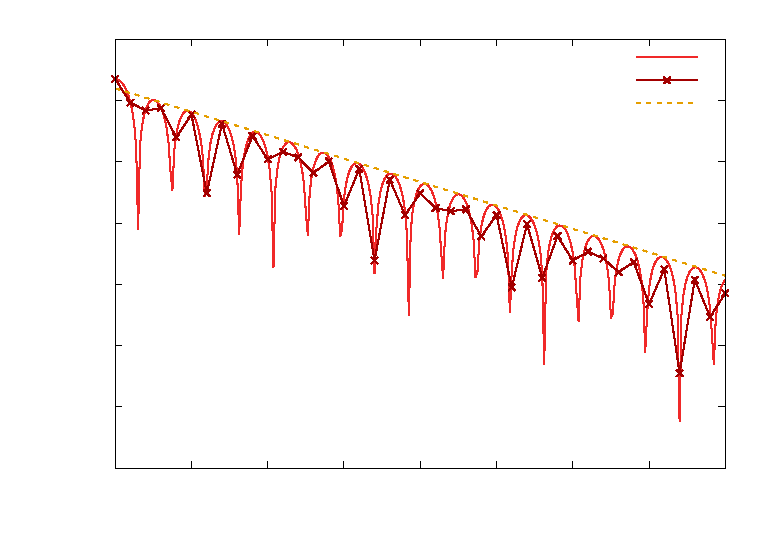
\includegraphics{img/Emax}}%
    \gplfronttext
  \end{picture}%
\endgroup
}
      \caption{Landau damping test: time history of $\|E(t)\|_{L^2}$ (semi-log scale) obtained with Lawson($RK(4, 4)$) and WENO5 
      with $\Delta t=1/8$ and $\Delta t=1$.}
      \label{ld}
    \end{figure}
  }
\end{frame}
%-------%
\begin{frame}{Bump on Tail (BoT)}
  $$
    f(t=0,x,v) = \left[\frac{0.9}{\sqrt{2\pi}}e^{-\frac{v^2}{2}} + \frac{0.2}{\sqrt{2\pi}}e^{-2(v-4.5)^2} \right](1+0.001\cos(0.5x))
  $$

  $x\in[0,20\pi]$, $v\in[-8,8]$, $N_x = 135$, $N_v=256$

  Numerical estimation of $\max_n||E^n||_\infty\approx 0.6$, we choose $\Delta t = \frac{C\Delta v}{0.6}$
\end{frame}
%-------%
\begin{frame}{BoT: numerical results}
  \only<1>{
    \begin{figure}
    \centering
        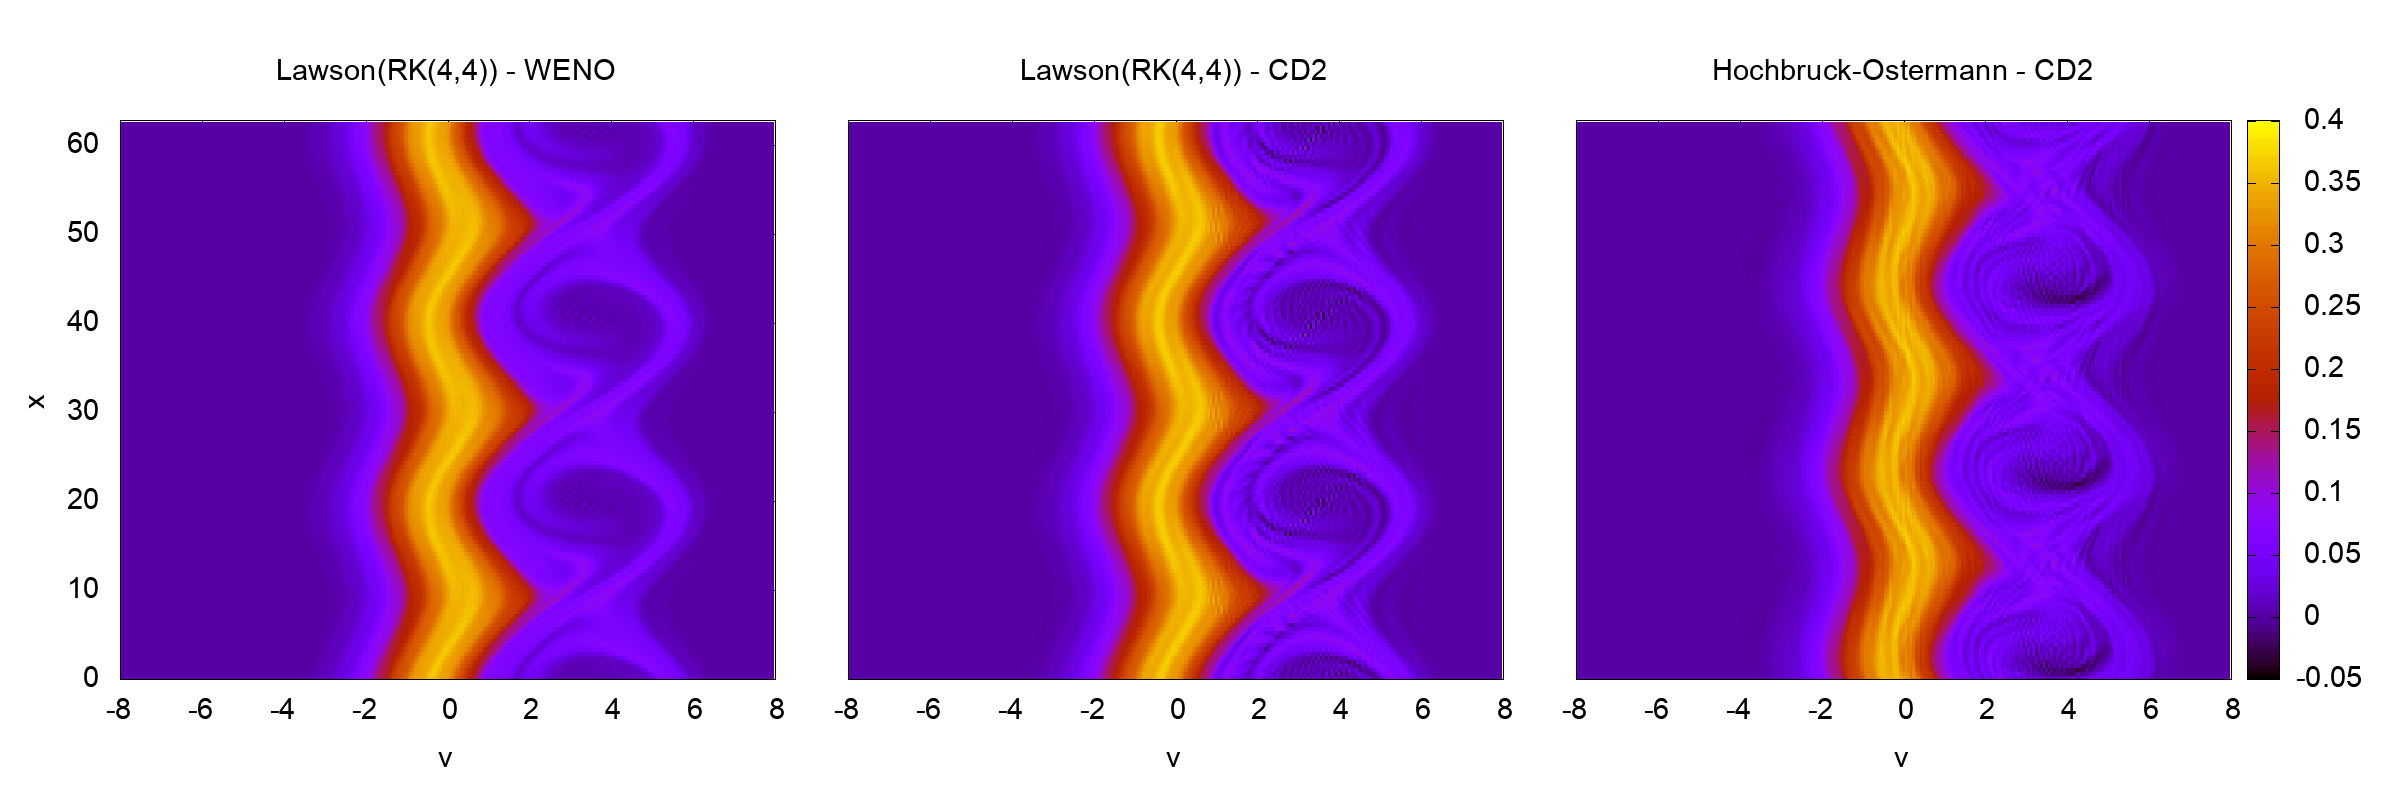
\includegraphics[width=\textwidth]{img/vp_cfl.png}
        \caption{Distribution function at time $t=40$ as a function of $x$ and $v$ for Lawson($RK(4, 4)$) + WENO5 (left), Lawson($RK(4, 4)$) + centered scheme (center), Hochbruck--Ostermann + centered scheme (right).}  
    \label{space}      
    \end{figure}
  } \only<2> {
    \begin{columns}
      \begin{column}{0.5\textwidth}
        \begin{figure}
          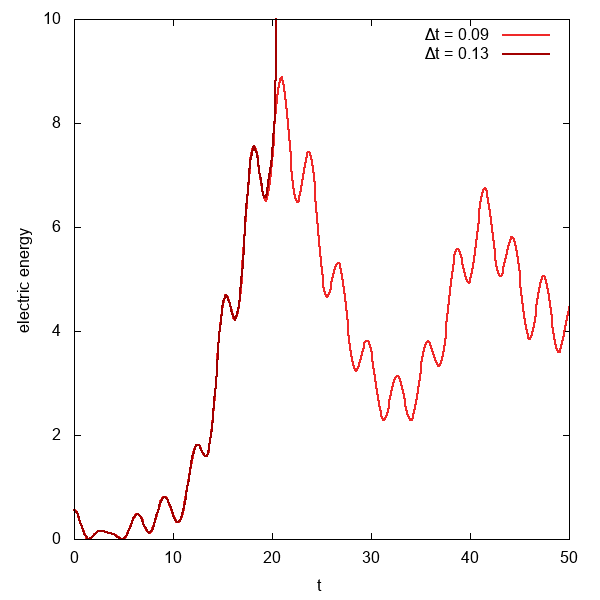
\includegraphics[width=0.9\textwidth]{img/ee_weno_rk44.png}
          \caption{Illustration of the accuracy of the CFL estimate obtained from the linear theory. History of electric energy with Lawson($RK(4,4)$) + WENO5}
        \end{figure}
        \vfill
        \ 
      \end{column}
      \begin{column}{0.5\textwidth}
        \begin{figure}
          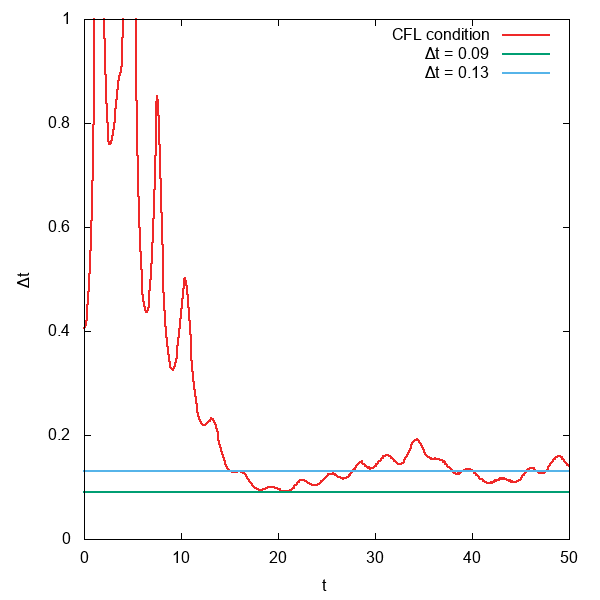
\includegraphics[width=0.9\textwidth]{img/bot_cfl_weno_rk44.png}
          \caption{History of CFL condition for Lawson($RK(4,4)$) + WENO5 case}
        \end{figure}
        \vfill
        \ 
      \end{column}
    \end{columns}
  } \only<3> {
    \begin{figure}
      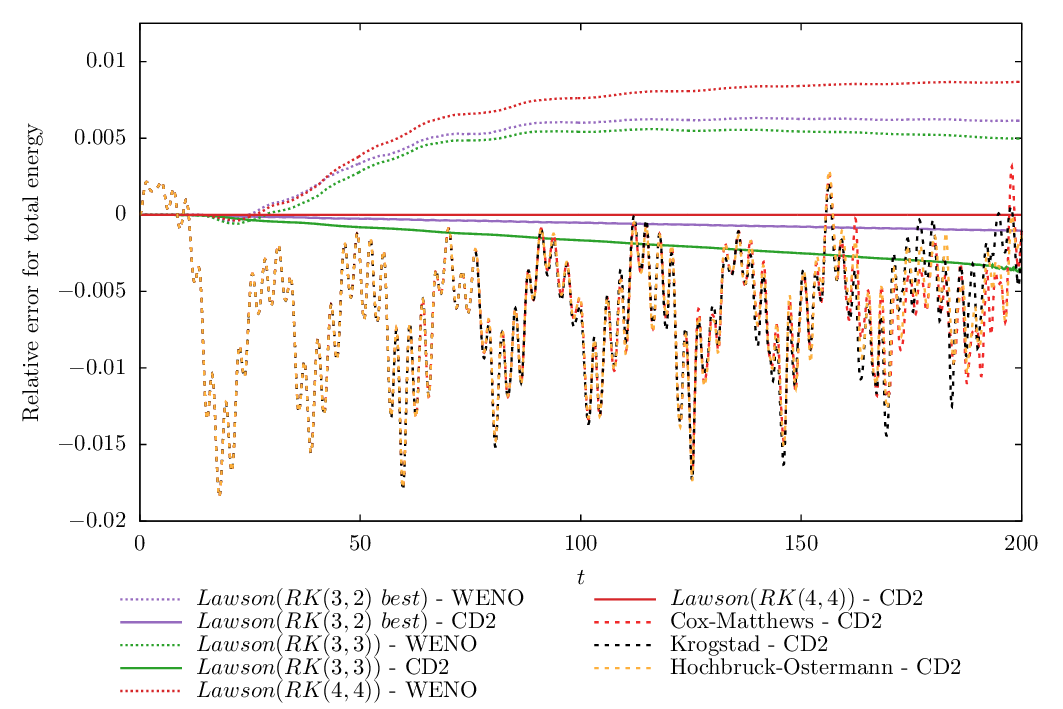
\includegraphics[width=0.9\textwidth]{img/H.png}
    \end{figure}
  }
\end{frame}
%-------%
\begin{frame}{Adaptive time step size}
  \centerline{\mbold{$\max_n||E^n||_\infty$ is not accessible in practice.}}

  \ 

  To capture correctly the phenomena involved in the bump on tail test, we take the following time step size:
  $$
    \Delta t_n = \min\left(0.1,\frac{C\Delta v}{||E^n||_\infty}\right)
  $$
  with $C=y_\text{max}$ or $\sigma$ from the linear theory.

  \arrow Good estimate in practice for Lawson methods.
\end{frame}



\section{Numerical simulation: drift-kinetic equations}
%%%%%%%%%%%%%%%%%%%%%%%%%%%%%%%%%%%%%%%%%%%%%%%%%%%%%%%%%%%%%%%%%%%%%%%%%%%%%%%

\begin{frame}{Drift-Kinetic equations}
  $f = f(t,r,\theta,z,v)$
  $$
    \begin{cases}
      \underbrace{\vphantom{\frac{}{}}\partial_tf + v\partial_zf}_{\text{linear part}} \underbrace{- \frac{\partial_\theta\phi}{r}\partial_rf + \frac{\partial_r\phi}{r}\partial_\theta f - \partial_z\phi\partial_vf}_{\text{non linear part}} = 0\\
      -\left[ \partial_r^2\phi + \left(\frac{1}{r}+\frac{\partial_rn_0(r)}{n_0(r)}\right)\partial_r\phi + \frac{1}{r^2}\partial_\theta^2\phi \right]+\frac{1}{T_e(r)}(\phi-\langle\phi\rangle) = \frac{1}{n_0(r)}\int_{\mathbb{R}}f\,\mathrm{d}v-1
    \end{cases}
  $$
  $(r,\theta,z,v)\in[0.1,14.5]\times[0,2\pi]\times[0,L]\times\mathbb{R}$

  After a Fourier transform in $z$, formally, the equation is still of the form of:
  $$
    \partial_t f + ikvf + F(f) = 0
  $$
  Compatible with all previous time integrators.

  This is more complicated to use linear stability analysis, we use an other adaptive time step method.
\end{frame}
%-------%
\begin{frame}{Adaptive time step size (error estimate)}
  For adaptive time step size with any time integrator $\varphi$:
  $$
    f^{n+1} = \varphi_{\Delta t_n}(f^n)\qquad;\qquad \tilde{f}^{n+1}=\varphi_{\Delta t_n/2}\circ\varphi_{\Delta t_n/2}(f^n)
  $$
  Richardson extrapolated numerical solution of the method of order $p$:
  $$
    f^{n+1}_R = \frac{2^{p+1}\tilde{f}^{n+1}-f^{n+1}}{2^{p+1}+1}
  $$
  estimate of the local error:
  $$
    e_{n+1} = || f^{n+1}_R - f^{n+1} ||_{L^\infty} + \mathcal{O}(\Delta t_n^{p+2})
  $$
  If $e_{n+1}>\text{tol}$: we reject the step and start again from time $t_n$. Else we determine the new time step size:
  $$
    \Delta t_{new} = s\Delta t_n\left(\frac{\text{tol}}{e_{n+1}}\right)^{1/(p+1)}
  $$
  $s=0.8$ is safety factor.
\end{frame}
%-------%
% \begin{frame}{Ion temperature gradient instability}
%    $$f(t=0,r,\theta,z,v) = f_{\text{eq}}(r,v)\left[1+\epsilon\exp\left(-\frac{(r-r_p)^2}{\delta r}\right)\cos\left(\frac{2\pi n}{L}z+m\theta\right) \right],$$
%     where the equilibrium (depends on space) distribution is given by:
%     $$
%       f_{\text{eq}}(r,v) = \frac{n_0(r)\exp\left(-\frac{v^2}{2T_i(r)}\right)}{(2\pi T_i(r))^{1/2}}
%     $$
% \end{frame}
%-------%
\begin{frame}{Ion temperature gradient instability: numerical results}
    \begin{figure}\centering
      \includegraphics[height=0.85\textheight]{img/{driftkinetic-tol1.00e-02-64x64x64x128-pert0}.pdf}
    \end{figure}
\end{frame}

\section{Conclusion}
%%%%%%%%%%%%%%%%%%%%%%%%%%%%%%%%%%%%%%%%%%%%%%%%%%%%%%%%%%%%%%%%%%%%%%%%%%%%%%%

\begin{frame}{Conclusion}
  \mbold{Summary}
  \begin{itemize}
    \item Better understanding on stability of Lawson or ExpRK methods in transport equations
    \item Python script with \texttt{sympy} to compute estimates of CFL of Lawson -- CD2, Lawson -- WENO (5 or 3) or ExpRK -- CD2 (with relaxing CFL)
    \item An adaptive time step size which works with any time integrators
  \end{itemize}

  \mbold{Future works}
  \begin{itemize}
    \item We can improve method with an embedded Runge-Kutta method (Dormand-Prince method, used in \texttt{ode45} of Matlab)
    \item Compare performance between exponential integrators and splitting methods (same stages/step, same order?)
    \item Use semi-Lagrangian method to remove dependency on periodic space (Fourier transform)
  \end{itemize}
\end{frame}

\begin{frame}[t]
  \vfill
  {\usebeamerfont{title} Thank you for your attention}
  \vfill
\end{frame}

%%%%%%%%%%%%%%%%%%%%%%%%%%%%%%%%%%%%%%%%%%%%%%%%%%%%%%%%%%%%%%%%%%%%%%%%%%%%%%%
\appendix
\backupbegin

\begin{frame}[plain]
  \vspace{0.65\textwidth}
  \hfill\footnotesize{Backup}
\end{frame}
%-------%
\begin{frame}{WENO5 method}
  \only<1>{
    \textbf{W}eighted \textbf{E}ssentially \textbf{N}on-\textbf{O}scillatory method of order 5: 3 estimates on 3 different stencils weighted with nonlinear weights.

    \begin{center}
      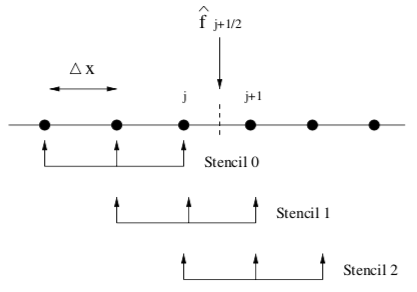
\includegraphics[width=0.5\textwidth]{img/stencils.png}
    \end{center}

    3 steps: \begin{enumerate}\item Indicator of smoothness \item Weights \item Flux \end{enumerate}
  }
  \only<2>{
    \mbold{Indicator of smoothness $\beta^\pm_i$}

    To approximate $\partial_xf(u)$:

    Split $f$ as:
    $$
      f(u) = f^+(u) + f^-(u)\quad,\quad \frac{df^+}{du}\geq 0\ \text{et}\ \frac{df^-}{du}\leq 0
    $$

    Indicators of smoothness:
    $$
      \beta_i^\pm  \gets (f^\pm_{[\![j-2,j+3]\!]})\ ,\ i=0,1,2
    $$
    Approximations of derivatives of order 1 and 2 on 3 stencils.
  }
  \only<3>{
    $$
      \begin{aligned}
        \beta_0^+ &= \frac{13}{12}\left( f^+_{j-2} - 2f^+_{j-1} + f^+_{j}   \right)^2\!\!\!\!\!\!&+& \frac{1}{4}\left(  f^+_{j-2} - 4f^+_{j-1} + 3f^+_{j}   \right)^2 \\
        \beta_1^+ &= \frac{13}{12}\left( f^+_{j-1} - 2f^+_{j}   + f^+_{j+1} \right)^2\!\!\!\!\!\!&+& \frac{1}{4}\left(  f^+_{j-1}              -  f^+_{j+1} \right)^2 \\
        \beta_2^+ &= \frac{13}{12}\left( f^+_{j}   - 2f^+_{j+1} + f^+_{j+2} \right)^2\!\!\!\!\!\!&+& \frac{1}{4}\left( 3f^+_{j}   - 4f^+_{j+1} +  f^+_{j+2} \right)^2\\
        & & & \\
        \beta_0^- &= \frac{13}{12}\left( f^-_{j+1} - 2f^-_{j+2} + f^-_{j+3} \right)^2\!\!\!\!\!\!&+& \frac{1}{4}\left( 3f^-_{j+1} - 4f^-_{j+2} +  f^-_{j+3} \right)^2 \\
        \beta_1^- &= \frac{13}{12}\left( f^-_{j}   - 2f^-_{j+1} + f^-_{j+2} \right)^2\!\!\!\!\!\!&+& \frac{1}{4}\left(  f^-_{j}                -  f^-_{j+2} \right)^2 \\
        \beta_2^- &= \frac{13}{12}\left( f^-_{j-1} - 2f^-_{j}   + f^-_{j+1} \right)^2\!\!\!\!\!\!&+& \frac{1}{4}\left(  f^-_{j-1} - 4f^-_{j}   + 3f^-_{j+1} \right)^2
      \end{aligned}
   $$
  }
  \only<4>{
    \mbold{Weights $w^\pm_i$}

    Unnormalized weights:
    $$
      \alpha_i^\pm \gets \frac{\gamma_i}{(\epsilon+\beta_i^\pm)^2}\ ,\  \gamma_i \in\mathbb{R}^*_+\,: \sum_k\gamma_k = 1
    $$
    where $\gamma_0 = \frac{1}{10}, \gamma_1=\frac{6}{10}, \gamma_2=\frac{3}{10}$. Parameter $\epsilon = 10^{-6}$

    Linearized weights (LW5): $\alpha_i^\pm = \gamma_i + \mathcal{O}(\Delta x^2)$

    Normalized weights:
    $$
        w_i^\pm \gets \frac{\alpha_i^\pm}{\sum_k\alpha_k^\pm}
    $$
  }
  \only<5>{
    \mbold{Flux $f^\pm_{i+\frac{1}{2}}$}

    $$
      \begin{aligned}
        f_{j+\frac{1}{2}}^+ \gets w_0^+ \left( \frac{2}{6}f^+_{j-2} - \frac{7}{6}f^+_{j-1} + \frac{11}{6}f^+_{j}\right)
                                + w_1^+ \left(-\frac{1}{6}f^+_{j-1} + \frac{5}{6}f^+_{j}   +  \frac{2}{6}f^+_{j+1}\right) \\
                                + w_2^+ \left( \frac{2}{6}f^+_{j}   + \frac{5}{6}f^+_{j+1} -  \frac{1}{6}f^+_{j+2}\right)
      \end{aligned}
    $$

    $$
      \begin{aligned}
        f_{j+\frac{1}{2}}^- \gets w_2^- \left(-\frac{1}{6}f^-_{j-1} + \frac{5}{6}f^-_{j}   + \frac{2}{6}f^-_{j+1}\right)
                                + w_1^- \left( \frac{2}{6}f^-_{j}   + \frac{5}{6}f^-_{j+1} - \frac{1}{6}f^-_{j+2}\right) \\
                                + w_0^- \left(\frac{11}{6}f^-_{j+1} - \frac{7}{6}f^-_{j+2} + \frac{2}{6}f^-_{j+3}\right)
      \end{aligned}
    $$

    $$
    \boxed{
      (\partial_x f(u))_j \approx \frac{1}{\Delta x}\left[(f_{j+\frac{1}{2}}^+ - f_{j-\frac{1}{2}}^+) + (f_{j+\frac{1}{2}}^- - f_{j-\frac{1}{2}}^-)\right]
      }
    $$
  }
\end{frame}
%-------%
\begin{frame}{More Lawson methods}
  \only<1>{
    We are interested in the numerical cost $\dfrac{\Delta t}{s}$ of RK($s$,$n$). To compare each time integrator, we compute total energy in Vlasov-Poisson system:
    $$
      H(t) = \int_{\Omega}\int_{\mathbb{R}} v^2f\,\mathrm{d}x\mathrm{d}v + \int_{\Omega}E^2\,\mathrm{d}x
    $$
    which is preserved in time. We propose to select the best method by considering:
    $$
      h_{s,n}:\frac{\Delta t}{s}\mapsto \left|\left| \frac{H(t)-H(0)}{H(0)} \right|\right|_{\infty}
    $$
  } \only<2> {
    \begin{figure}\centering
      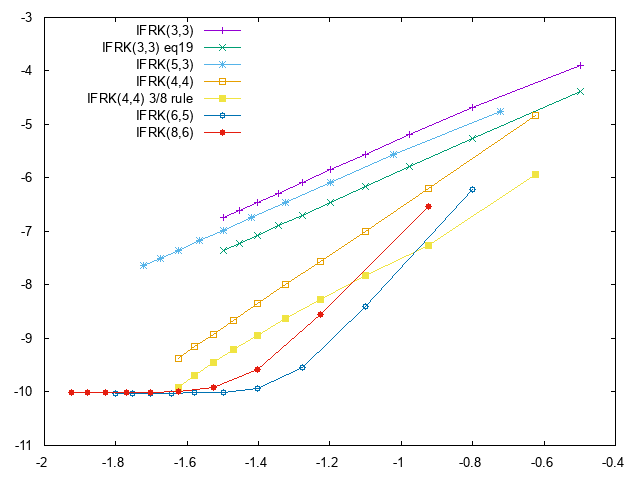
\includegraphics[height=0.8\textheight]{img/oHdt.png}
    \end{figure}
  }
\end{frame}

\backupend
%%%%%%%%%%%%%%%%%%%%%%%%%%%%%%%%%%%%%%%%%%%%%%%%%%%%%%%%%%%%%%%%%%%%%%%%%%%%%%%

\end{document}
